\subsection{RESULTADOS DE LAS DIFERENTES VARIANTES DE LA CADENA}
\subsubsection{Métricas separadas}
Primero se evalúa el impacto de las diferentes métricas por separado según las diferentes configuraciones. 
Al comparar la mejora de PESQ respecto a la reducción del dataset Figura \ref{fig:horas_vs_pesq}, se observa que 

Primero es compara la relación entre calidad de audio y cantidad de horas del dataset. La Figura \ref{fig:horas_vs_pesq} muestra, en el eje horizontal, el porcentaje de reducción del dataset producido por el filtrado (más a la derecha significa pérdida de más horas) y, en el eje vertical, el incremento relativo de la puntuación PESQ expresado en porcentaje. Sobre la misma gráfica se comparan las tres variantes de la etapa de realce consideradas: DeepFilterNet, Demucs y la condición sin denoise. El comportamiento observado evidencia un trade-off claro entre cantidad y calidad: umbrales de filtrado más estrictos producen mejoras mayores en PESQ pero sacrifican un mayor número de horas de grabación. En concreto, las variantes con denoising aportan ganancias moderadas en PESQ (típicamente inferiores al 8\% según el umbral), mientras que la variante sin realce logra aumentos mayores en PESQ (superiores al 10\%) a costa de una reducción de dataset mucho más agresiva. Entre los métodos de realce usados, Demucs tiende a ofrecer las mayores mejoras de PESQ a lo largo de los umbrales evaluados, y DeepFilterNet presenta ganancias más pequeñas para filtros equivalentes; esta diferencia implica que la elección del algoritmo de realce y del umbral de NISQA debe hacerse en función del balance deseado entre calidad perceptual y preservación de horas útiles.

\begin{figure}[h]
  \centering
  \centerline{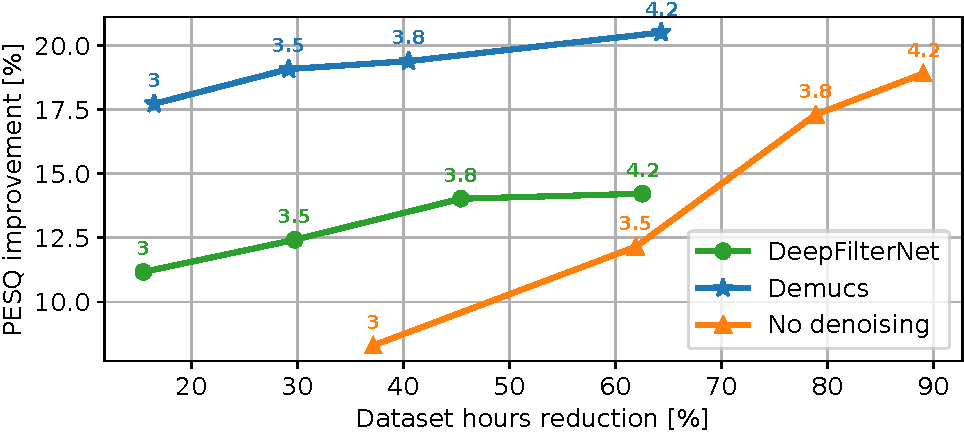
\includegraphics[width=15cm]{Figuras/Pipeline/pesq vs horas bien.pdf}}
  \caption{Comparación entre PESQ y cantidad de horas de las variantes.}
    \label{fig:horas_vs_pesq}
\end{figure}

La Figura 3 relaciona la reducción porcentual de horas con la mejora relativa en \(T_{30}\) (tiempo de reverberación estimado) cuando se emplea DNSMOS como métrica de filtrado. En la gráfica, un aumento en la mejora de \(T_{30}\) implica una reducción de la energía tardía y, por ende, una menor reverberación aparente en los segmentos retenidos. Los resultados muestran que el filtrado aporta ganancias en condiciones sin denoise de forma especialmente notable —es decir, cuando no se aplica realce previo el filtrado selecciona segmentos con menor reverberación y la mejora en \(T_{30}\) es sustancial—; en las condiciones ya denoised las ganancias en \(T_{30}\) son más moderadas (por debajo aproximadamente del 5\% en los umbrales considerados). Además, no se detecta una diferencia significativa en \(T_{30}\) entre DeepFilterNet y Demucs, aunque Demucs presenta una ventaja apreciable (alrededor de 5\%) en medidas de claridad como \(C_{50}\). En conjunto, la figura subraya que el filtrado basado en DNSMOS puede reducir la reverberación del subconjunto resultante, pero el beneficio marginal depende fuertemente de si previamente se aplicó un algoritmo de realce y de la agresividad del umbral. :contentReference[oaicite:1]{index=1}


La Figura 4 ilustra la relación entre la mejora relativa de PESQ (eje horizontal) y la diferencia porcentual en la desviación estándar de \(F0\) (\(F0\text{-}STD\), eje vertical) para las variantes evaluadas con DNSMOS. Esta representación revela un efecto colateral relevante: a medida que aumenta la mejora perceptual (PESQ) por filtrado más estricto, suele observarse una reducción de la variabilidad prosódica medida por \(F0\text{-}STD\). La explicación práctica es que el filtrado agresivo tiende a eliminar segmentos y hablantes de peor calidad, lo cual reduce la heterogeneidad prosódica del subconjunto retenido. No obstante, los métodos de realce que mejor preservan el timbre de voz muestran cambios menores en \(F0\text{-}STD\) ante el mismo grado de filtrado, lo que indica que ciertos denoisers permiten mejorar la calidad percibida sin sacrificar tanto la variabilidad prosódica. En la práctica, la figura pone de manifiesto el compromiso entre mejorar la calidad objetiva del audio y mantener la diversidad de patrones de entonación: selección excesiva orientada únicamente a PESQ puede empobrecer la variabilidad del corpus, con posible impacto en tareas de síntesis que requieran conservar rasgos prosódicos y de identidad. Además, en el paper se reporta que la MCD varía poco con el filtrado y que Demucs típicamente obtiene una MCD algo menor que DeepFilterNet, lo que refuerza la recomendación de evaluar simultáneamente métricas de calidad y métricas de preservación vocal antes de fijar una configuración final. :contentReference[oaicite:2]{index=2}


\subsubsection{Métricas conjunta}
Hacer el ranking de todas las variantes según el resultado de optimización.

\subsection{COMPARACIÓN ENTRE CONJUNTOS DE DATOS}
Comparar entre conjuntos de datos profesionales vs datos ITW (por parametros acústicos)

\subsection{COMPARACIÓN POR ESTIMACIÓN DE DENSIDAD}
Comparar entre conjuntos de datos profesionales vs datos ITW (por estimación de densidad)

\subsection{VALIDACIÓN MODELO DE TTS ZERO-SHOT}
Compara calidad de clonación respecto a la calidad o subset del audio original
